%\section{Basics of Cybersecurity}\label{ch:basics_cybersec}
%This chapter briefly explains the terms of IT security and cybersecurity and gives an overview of their goals and methods.
%A summary of common threats in the cyberspace is given as well, giving context for \cref{ch:testing}.
%
%\section{IT Security}
%IT Security describes the protection of digital data and computer- and communication systems from unauthorized access.
%Different principles are adhered to and methods and techniques applied in order to prevent the theft, interception, manipulation, and loss of data and systems. \cite{IT_Basiswissen}
%
%\section{Cybersecurity}
%IT- and cybersecurity are similar in that both have the same goals and apply the same principles and methods.
%While IT Security focuses on classical computer systems and networks, cybersecurity focuses on data and systems in the cyberspace.
%Included in the cyberspace are all systems and data connected to the internet.
%
%\subsection{Goals}
%The goals of cybersecurity include but are not limited to the well-known CIA triad, which is an acronym for Confidentiality, Integrity, and Availability \cite{Oriyano_2017}.
%Confidentiality describes data only being accessible by the persons who are meant to do so.
%Integrity describes data being unchanged after storage or transmission, meaning the data was not corrupted or manipulated.
%Availability describes data and systems being accessible with the expected performance, whenever required. 
%
%\subsection{Methods}\label{ssec:cs_methods}
%Some methods for achieving the goals of cybersecurity are:
%
%\begin{itemize}
%    \item Security Awareness is the knowledge of the threats present in the cyberspace and methods for protection.
%    "Awareness of the risks and available safeguards is the first line of defence for the security of information systems and networks" \cite[page~26]{IT_Basiswissen}.
%    \item Encryption is a cryptographic\footnote{cryptography = science of secretive writing} method, which takes the readable data, called plaintext, and makes it unreadable for anyone besides the legitimate recipient.
%    The encrypted text is called ciphertext and can be made readable again by decrypting it.
%    To en- and decrypt a message, the sender and recipient have knowledge of a secret, often a password, which controls en-/decryption and is called key. \cite[page~1]{Watjen_2018}
%    \item Authentication is the act of a user "performing some sort of action which proves that the claim a user is making about who they are is actually valid" \cite{Oriyano_2017}. 
%    This is oftentimes done through the use of a password, in the case of Wi-Fi networks, the knowledge of the password proves that a user is allowed to access the network.
%    \item Pentesting is a method to audit the security of a system or network. 
%    It involves a security professional performing various types of attacks to discover weaknesses in soft- and hardware.
%    \item Monitoring with anomaly detection can be used to detect the unauthorized access of systems and networks.
%    In the network domain, so-called Intrusion Detection Systems (IDS) employ predictive models to recognize malicious activity inside a network \cite{geeksforgeeks_ids}.
%    \item Incident Response is performed in case of a system breach in order to limit damage and secure the system.
%\end{itemize}
%
%\section{Threats and Risks in the Cyberspace}
%There are various types of cybercriminals with different motives and intentions.
%Motives of cybercriminals can vary, but commonly are financial, political, social, or military.
%With these motives the intentions of an attack often are:
%\begin{multicols}{2}
%    \begin{itemize}
%        \item blackmail
%        \item espionage
%        \item theft
%        \item fraud
%        \item sabotage
%        \item corruption and insider deals
%    \end{itemize}
%\end{multicols}
%
%The success rate and risk of an attack are in large parts determined by a target's attack area, which is the combination of the present vulnerabilities and attack vectors.
%The term vulnerability describes a weak spot, which can be exploited by the attacker to break or circumvent security mechanisms.
%An attack vector is the approach an attacker takes for carrying out an attack.
%In regard to network security some common attack vectors are:
%
%\begin{itemize}
%    \item Denial of Service (DoS) attacks availability by preventing or limiting the functional capability of a system.
%    \item Cracking describes the act of breaking or circumventing security mechanisms, e.g. reverse engineering passwords.
%    \item Brute-Force is a technique for reverse engineering passwords by trail-and-error.
%    \item Dictionary attack is a variation of Brute-Force, using a collection of leaked passwords to guess the correct solution.
%    \item Spoofing refers to faking identities, achieved by the obfuscation of the own identity or the replication of another identity.
%    \item Sniffing is the action of collecting all openly available data, e.g. recording unencrypted Wi-Fi frames.
%    \item Man-in-the-Middle (MitM) attacks involve injection of a malicious device into a line of communication, which subsequently can manipulate and eavesdrop on the traffic.
%    \item Social Engineering is a form of manipulation that abuses psychological mechanisms like trust, curiosity, or shock to exploit victims.
%\end{itemize}
%
%\cite[page~16-20]{IT_Basiswissen}
{
\section{Einführung Cybersecurity}
\begin{frame}
    \centering
    \tableofcontents[currentsection]
\end{frame}

\begin{frame}{Bedrohungen}
    \small
    \begin{columns}

        \begin{column}{0.3\textwidth}
            \textbf{Motiv}
            \begin{itemize}
                \item finanziell
                \item politisch 
                \item sozial 
                \item militärisch
            \end{itemize}
        \end{column}\pause

        \begin{column}{0.3\textwidth}
            \textbf{Absicht}
            \begin{itemize}
                \item Erpressung
                \item Spionge
                \item Diebstahl
                \item Betrug
                \item Sabotage
                \item Korruption
            \end{itemize}
        \end{column}\pause

        \begin{column}{0.3\textwidth}
            \textbf{Angriffsvektor}
            \begin{itemize}
                \item Malware
                \item Social Engineering
                \item Denial of Service (DoS)
                \item Cracking
                \item Spoofing
                \item Man-in-the-Middle (MitM)
            \end{itemize}
        \end{column}

    \end{columns}
\end{frame}

\begin{frame}{Ziele von Cybersecurity - CIA Acronym}
    \small
    \begin{columns}
        \begin{column}{0.3\textwidth}
            \begin{flushright}
                {\large\textbf{Vertraulichkeit}}
                \\Information ist nur für berechtigte Personen lesbar
                \vspace{3cm}
            \end{flushright}
        \end{column}

        \begin{column}{0.4\textwidth}
            \begin{center}
                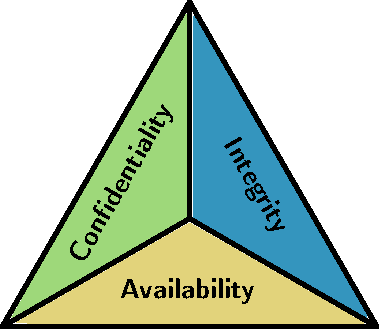
\includegraphics[height=.5\textheight]{figures/CIA.pdf}
            \end{center}
            {\large\textbf{Verfügbarkeit}}
            \\Daten und Services sind mit benötigter Leistung zum benötigten Zeitpunkt verfügbar
            \vspace{0.5cm}
        \end{column}

        \begin{column}{0.3\textwidth}
            {\large\textbf{Integrität}}
            \\Information ist unverfälscht
            \vspace{3cm}
        \end{column}
    \end{columns}
\end{frame}

\begin{frame}{Schutzstrategien}
    \large
    \begin{columns}
        \begin{column}{1cm}
        \end{column}
        \begin{column}{8cm}
            \begin{itemize}
                \setlength{\itemsep}{10pt}
                \item Security Awareness 
                \item Sicherheitsarchitekur
                \item Verschlüsselung
                \item Authentifizierung
                \item Pentesting 
            \end{itemize}
        \end{column}
    \end{columns}
\end{frame}
}